

\typeout{An AI Success Story in Metaphysics: \\ the Case of the Inconsistency in G\"odel's Ontological Argument}


\documentclass{article}
\usepackage{ijcai15}

% Use the postscript times font!
\usepackage{times}


% the following package is optional:
\usepackage{latexsym} 

\usepackage{amsmath}
\usepackage{xspace}
\usepackage{modallogics}
\usepackage{graphicx,url}
\usepackage{txfonts} % needed for \Diamondblack
\usepackage{color}
\usepackage{xcolor}

\newcommand{\imp}{{\rightarrow}}
\newcommand{\biimp}{\leftrightarrow}
\newcommand{\allq}{\forall}
\newcommand{\exq}{\exists}
\newcommand{\seq}{\vdash}

\newcommand{\Dia}{\Diamond} % possibly
\newcommand{\BlackBox}{\blacksquare}
\newcommand{\BlackDia}{\Diamondblack}

\newcommand{\NE}{\mathit{NE}}
\newcommand{\ess}[2]{#1\ \mathit{ess}\ #2}
\newcommand{\nec}{\Box}
\newcommand{\pos}{\Dia}


\title{An AI Success Story in Metaphysics: \\ the Case of the Inconsistency in G\"odel's Ontological Argument}
\author{Christoph Benzm\"uller\thanks{German Research Foundation DFG \ldots} and Bruno Woltzenlogel Paleo}
\author{}

\begin{document}

\maketitle

\begin{abstract}
  This paper discusses the discovery of the inconsistency in G\"odel's ontological argument as a success story for artificial intelligence. Despite the popularity of the argument since the appearance of G\"odel's manuscript in 1970, the inconsistency of the axioms used in the argument remained unnoticed until 2013, when it was detected automatically by the higher-order theorem prover \textsc{Leo-II}. Understanding and verifying the refutation generated by the prover turned out to be a time-consuming task, and its completion, as reported here, required the reconstruction of the refutation in the Isabelle proof assistant. The development of an improved syntactical hiding for the embedding technique, utilizing Isabelle's binding notation mechanism, allows the refutation to be presented in a human-friendly way, suitable for non-experts in the technicalities of higher-order theorem proving. This brings us a step closer to wider adoption of logic-based artificial intelligence tools by philosophers.
\end{abstract}


\section{Introduction}\label{sec:introduction}
Without exaggeration Kurt G\"{o}del's ontological
argument for the existence of God \cite{GoedelNotes,ScottNotes} is
amongst the most discussed formal proofs in modern literature. A rich
body of publications -- including very recent ones -- present,
discuss, assess, criticise, modify and improve G\"{o}del's original
work (see e.g.~Sobel~\shortcite{sobel2004logic} and Oppy~\shortcite{sep-ontological-arguments} and the
references therein).  In philosophy lectures at universities the
argument is regularly presented as a masterpiece argument in
metaphysics. Since 2013, when Benzm\"uller and Woltzenlogel-Paleo~\shortcite{J30,C40} first
reported their successful initial computer-assisted
analysis of G\"odel's proof and Scott's variant,
their work has received a media repercussion on a global scale\footnote{A
  small collection of news articles is available at {\scriptsize
    \url{https://github.com/FormalTheology/GoedelGod/blob/master/Press/LinksToNews.md}}},
and numerous bloggers commented on the proof
\cite{fuhrmann15:_blogg_goedel}.

The in-depth computational analysis presented here substantially
extends previous computer-assisted studies of G\"odel's ontological
argument. Similar to the related work \cite{J30,C40} the analysis has
been conducted with automated theorem provers for classical
higher-order logic (HOL; cf. \cite{andrewsSEP} and the references
therein) even though G\"odel's proof is actually formulated in
higher-order \emph{modal} logic (HOML; cf. \cite{homl} and the
references therein). To bridge between the two logics we utilise and
further improve the logic embedding approach \cite{J23,C40}, which has
already been employed successfully in preceding related work.

The main novel contribution reported in this paper is a detailed
analysis (in various modal logics) of the inconsistency of G\"{o}del's
original version of the axioms used in his proof
\shortcite{GoedelNotes}. The extraction, reconstruction and
verification of an informal, human intuitive argument has been an open
problem since the first detection of this inconsistency by
Benzm\"uller and Woltzenlogel-Paleo \shortcite{C40} with the
\textsc{Leo-II} prover.  The verified refutation (discussed in
\S\ref{sec:inconsistency}) displays a surprisingly accessible
explanation of the inconsistency, which is philosophically profound
and never presented in the literature. The detection of this
inconsistency in combination with the work reported here thus
demonstrates that artificial intelligence systems -- particularly
higher-order automated theorem provers -- are capable of assisting in
the discovery and elucidation of \emph{new} and philosophically
relevant knowledge.

On the technical side, the quest for constructing a compelling
refutation, capable of convincing also human non-experts, led us to
improve the syntax of the embedding of modal logics in Isabelle/HOL
(as discussed in \S\ref{sec:improvedsyntax}). With the new syntax, a
(nearly) perfect match between the original pen and paper
presentations and our encoding in Isabelle/HOl is feasible. A more
user-friendly syntax, as reported here, is clearly an important
prerequisite for promoting the theorem proving technology employed
here to a wider community of philosophers, who are not necessarily
experts in automated reasoning or higher-order logic.

Another novel contribution reported here (in \S\ref{sec:improvedembedding}) is
the implementation of an alternative embedding for the only slightly
stronger modal logic \SFiveU. Our experiments have shown that the new
embedding is more efficient, as the following two, previously open problems can now be solved:
\begin{itemize}
\item Proving the final theorem T3 \textit{``Necessarily, there
    exists God''} (in Scott's \shortcite{ScottNotes} consistent variant) fully automatically and directly from the axioms
  alone, without relying on the argument's intermediate argumentation
  steps (i.e., lemmata).
\item Verifying automatically (in Isabelle/HOL) the proof of the modal
  collapse \cite{Sobel}, which is one of the most strongly criticized
  `side-effects' of the argument's axioms.
\end{itemize}


\subsection{Related Work}

First successful applications of theorem proving technology in
metaphysics were reported by Oppenheimer and
Zalta~\shortcite{oppenheimer11}, who coined the term \textit{Computational Metaphysics} for this new research area and employed the first-order
\textsc{Prover9} \cite{prover9-mace4} in their experiments. Later on, Rushby~\shortcite{rushby13} used the proof assistant \textsc{PVS} \cite{cade92-pvs}. Common to both
works is a significant amount of proof-hand-coding work as well as their
focus on a non-modal formalization of St. Anselm's~\shortcite{Proslogion} simpler 
and older ontological argument. 
None of these previous works formalises and automates variants of \emph{higher-order} and \emph{modal} logics, which are, however, crucial
for G\"{o}del's more complex ontological argument.


\section{A Brief History of the Argument}\label{sec:history}

St. Anselm's ontological argument \cite{Proslogion} can be regarded as
the ancestor of modern ontological arguments such as G\"odel's. In the
millenium between Anselm and G\"odel, many philosophers modified and
arguably improved Anselm's argument. Of particular importance to
G\"odel was the work of Leibniz \cite{ToDo:Leibniz}.  G\"odel's manuscript
(Fig.~\ref{GoedelScript}) can be considered a translation of Leibniz's
presentation of the argument into modern modal logic. G\"odel
discussed his manuscript with Scott, who shared a slightly different
version with a larger public. Scott's version of the axioms and
definitions, formalized in Isabelle, is shown in
Fig.~\ref{Scott_S5U}. The main difference to G\"odel's version is the
addition of a conjunct in the definition of \emph{essence}. G\"odel's
different definition of essence can be seen either in his manuscript
(Fig.~\ref{GoedelScript}) or, in more modern notation, in the Isabelle
formalization shown in Fig.~\ref{InconsistencyIsabelleK}. For Scott,
an essential property of an individual must be possessed by
him/her. For G\"odel, this is not required. This difference has been
considered inessential and merely an oversight by many. For instance,
Hazen 1998, p.365 \cite[p.365]{Hazen} states that ``G\"odel left this
clause out in [11], but this appears to have been an oversight--it is
included in related manuscripts''. However, the omitted conjunct is in
fact crucial. Without it, G\"odel's original axioms are
inconsistent. With it, Scott's axioms are consistent (cf.~Fig.~\ref{Scott_S5U}
where the model finder Nitpick \cite{Nitpick} confirms consistency).\footnote{In
  personal communication, Dana Scott confirmed that he was unaware
  that G\"odel's axioms were inconsistent.}


% There is reason to believe that the omission was more than just an oversight. As pointed out by Fuhrmann \cite{Fuhrmann2005}, ``G\"odel vermerkt diese Konsequenz [dass aus der Definition unmittelbar folgt, da\ss alle wesentlichen Eigenschaften notwendig äquivalent sind] in einer Fußnote zur Definition. Die Definition selbst aber l\"a{\ss}t im Definiens das Konjunkt $Xx$ aus. Ohne das Konjunkt folgt jedoch die Konsequenz nicht. Es ist deshalb naheliegend anzunehmen, da\ss G\"odel die Definition so beabsichtigte, wie sie hier notiert ist und wie G\"odel sie selbst in fr\"uheren Notizbucheintragungen formuliert hat.''\footnote{Our translation: ``G\"odel remarks this consequence [that the definition of essence entails that all essences are necessarily equivalent] in a footnote to the definition. The definition, however, omits the conjunct. ... ToDo''} 
% \marginpar{ToDo: check Fuhrmann's claim. He may be pointing out a second mistake by Gödel.}

For more than four decades, the serious consequences of G\"odel's
mistake remained unnoticed, despite intense activity focused on
criticizing his argument. Especially since the discovery by Sobel
\cite{Sobel} that modal collapse (MC)\footnote{The modal collapse,
  $\phi\rightarrow \Box \phi$, states that contingent truth implies
  necessary truth; it can be interpreted as \textit{everything is
    pre-determined} or even \textit{there is no free will}. } is
entailed by G\"odel's (or also Scott's) axioms, several variants have
been proposed
\cite{Anderson,AndersonGettings,Hajek1,Hajek2,Hajek3,Bjordal}
attempting to avoid the modal collapse. Many of these variants omit
the crucial conjunct in the definition of essence as well\footnote{As
  these variants also change other axioms, on which the inconsistency
  of G\"odel's axioms depends, it is not necessarily the case that
  these variants are also inconsistent; each case needs to be analysed
  separately.}. Opponents of the argument
(e.g. Oppy \cite[p.226/227]{oppy96:_goedel_ontol_argum}
\cite[p.364]{oppy00:_respon_gettin}
\cite[p.1068]{oppy08:_higher_order_ontol_argum}) have also proposed
parodies and other criticisms, referring to variants where the
conjunct is omitted.





%  Particularly interesting
% from the perspective of this paper is that many literature
% contributions unfortunately work with or refer to G\"odel's original
% definition of essence
% $$ todo $$
% This original version avoids the conjunct added by Scott expressing
% that essential properties of an individual should be possessed by the
% individual. 

% We give here a list of examples:
% \begin{itemize}
% \item Anderson and Getting's 1996, p. 168 \cite[p.168]{AndersonGettings1968}
%   use essence without conjunct.
% \item  
% \item Look???, p. 514
% % \item Oppy 1996, p.226-227 \cite[p.226/227]{Oppy1996}, Oppy 2000, p. 364
% %   \cite[p.364]{Oppy200}, Oppy 2008, p. 1068 \cite[p.1068]{Oppy2008}:
% %   Oppy uses: ``A is an essence of x iff for every property B, x has B
% %   neces- sarily iff A entails B'' (this is from Anderson's
% %   emendation). Check is this leads to inconsistency as well. In this
% %   case we may write something like: 

% %  Oppy presents an critical
% %   assessment in order to conclude that G\"odel's argument fails to
% %   convince. Oppy apparently does not see that he is assessing an
% %   inconsistent axiom system (and he in fact creates adaptations that
% %   suffer the same problems).
% % \item 
% \end{itemize}








\section{Automating HOML in HOL}\label{sec:homlinhol}

Logic textbooks % \cite{ToDo:which}
commonly utilize higher-order logic in an informal/semi-formal way as
a meta-language to introduce the syntax and the semantics of object
logics of interest, in which reasoning problems in concrete
application domains can be modeled and solved with pen and paper. In
fact, this approach can also be followed on the computer (using HOL as
a formal meta-language) for even very challenging object logics (such
as HOML) to enable interactive and automated theorem proving with
existing theorem provers for HOL.

% Just as commonly the case in logic textbooks, in the embeddings
% approach classical higher-order logic is utilised as a meta-language
% to encode the syntax and the semantics of object logics in which the
% proof problems of interest are then modeled in. Modulo the embedding
% state of the art automated theorem provers for classical higher-order
% logic can then be utilised as object logic reasoning tools.

For a computational analysis of G\"odel's ontological argument in this
approach the embedding of HOMLs such as K,
KB and S5 with various domain conditions (possibilist and actualist)
is required. This idea has been successfully followed in related work
\cite{C40}. The embedding of HOML is in fact
straightforward. Formulas in HOML are \emph{lifted}, translated to predicates
over worlds, which are themselves explicitly represented as
terms. The logical constants of HOML are translated to HOL terms in such a way that, for instance, 
%$\neg \varphi$, $\varphi\vee\psi$
$\Box \varphi$ and $\Diamond \varphi$ (relative to a current world
$w_o$) are mapped, respectively, to the HOL formulas
$\forall w. (r w_0 w) \imp (\varphi w)$ and
$\exists w. (r w_0 w) \wedge (\varphi w)$. This form of embedding is
precisely the well-known standard translation
\cite{DBLP:journals/logcom/Ohlbach91}, which is here intra-logically
realized --- and extended for quantifiers --- in HOL by stating a set
of equations defining the logical constants (Fig.~\ref{QML_S5U}). The
resulting object logic is the HOML K with rigid terms and constant
domains (possibilist quantifiers). Other logics (e.g. KB, S5) can be
embedded by adding axioms that restrict the accessibility relation
$r$. Varying domains and actualist quantifiers can be simulated by
means of an existence predicate, which can be used to guard the
quantifiers. Therefore, the embedding approach is very flexible.


\subsection{Improved Embedding}\label{sec:improvedembedding}
\begin{figure}[t]
\centerline{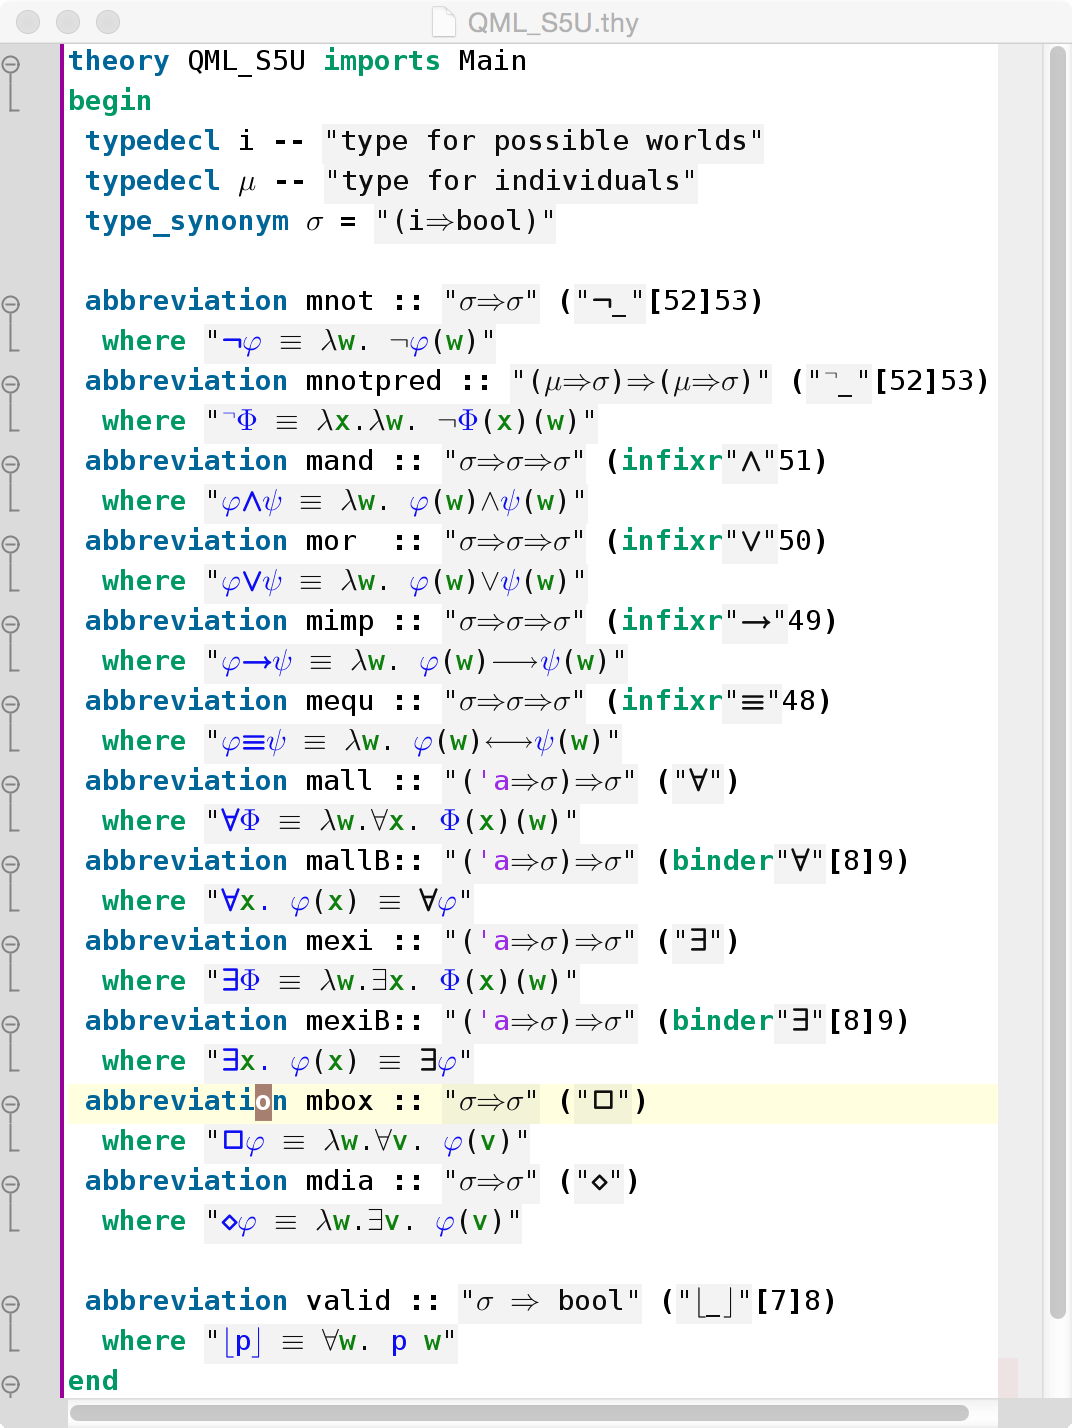
\includegraphics[width=\columnwidth]{./Images/QML_S5U.png}}
\caption{Improved Embedding of \SFiveU} \label{QML_S5U}
\end{figure}

The modal logic \SFive requires that the accessibility relation be
reflexive, symmetric and transitive. The usual approach to embed
\SFive would be to use the standard translation for K described above
and to state that $r$ is an equivalence relation, e.g., by postulating
the following axioms:
\begin{itemize}
\item Reflexivity: $\forall x. (r~x~x)$
\item Symmetry: $\forall x. \forall y. (r~x~y) \rightarrow (r~y~x)$ 
\item Transitivity: $\forall x. \forall y. \forall z. (r~x~y) \wedge (r~y~z) \rightarrow (r~x~z)$
\end{itemize}
Instead, we consider here a modal logic that we call \SFiveU, which is
characterized by the following condition on $r$:
\begin{itemize}
\item Universality: $\forall x. \forall y. (r~x~y)$
\end{itemize}

It is easy to see that \SFiveU is at least as strong as \SFive:
universality entails that $r$ is an equivalence relation. \SFiveU is,
in fact, \emph{strictly stronger} than \SFive. \SFiveU only admits
complete\footnote{A graph is \emph{complete} iff there is a directed
  edge connecting every ordered pair of vertices.} frames, whereas
\SFive admits non-complete frames as long as all their components are
complete. In other words, in \SFiveU we face one single equivalence
class of possible worlds, while in \SFive we may face several
disconnected equivalence classes. In fact, for this reason, \SFiveU is
considered as metaphysically more appropriate by some philosophers;
cf. \cite[p.~127]{williamson13}.

For \SFiveU, an improved embedding is possible. Universality implies
that the guarding predicates in the definitions of $\Box$ and
$\Diamond$ always hold. Therefore, they can be omitted and the
accessibility relation can be dispensed altogether. The modal
operators can then be defined merely as:
% \begin{itemize}
% \item $\BlackBox \varphi \equiv \forall w. (\varphi w)$ 
% \item $\BlackDia \varphi \equiv \exists w. (\varphi w)$
% \end{itemize}
\[\Box \varphi \equiv \lambda w. \forall v.  \varphi(v) \qquad \text{and}
\qquad \Dia \varphi \equiv \lambda w.\exists v. \varphi(v)\]


The new embedding of \SFiveU in Isabelle is shown in
Fig.~\ref{QML_S5U}. It is important to note that we 
have  $\vDash_{\SFive} \varphi$ iff $\vDash_{\SFiveU} \varphi$,
despite the differences in the underlying frame structures.


%
% \marginpar{@Bruno: I commented you paragraph here, since I am not
%   convinced (yet) that e.g. BF and CBF are equally valid in \SFiveU
%   and \SFive}
% \SFiveU is only slightly stronger than \SFive. Most importantly,
% $\vDash_{\SFive} \varphi$ iff $\vDash_{\SFiveU} \varphi^{U}$, where
% $\varphi^U$ is obtained from $\varphi$ by replacing all $\Box$ and
% $\Dia$ by, respectively, $\BlackBox$ and $\BlackDia$. Therefore,
% \SFiveU can be considered as adequate for metaphysics as \SFive
% (cf. \cite[p. 127]{WilliamsonModalLogicAsMetaphysics}). 
% % \cite{Mattey}, \cite[ToDo]{DunnHardegree}
%
With this improved embedding, the final theorem T3
(\textit{``Necessarily, there exists God''}) can be derived from
Scott's consistent version of the axioms fully automatically.  The fully
automatic proof has been generated (in about 2,5 seconds) by the theorem prover
\textsc{Leo-II}~\cite{C26} and subsequently verified in the proof
assistant Isabelle/HOL~\cite{NPW02}, as shown in Fig.~\ref{Scott_S5U}.
The collaboration between the two systems has been orchestrated by
Isabelle's Sledgehammer tool \cite{Sledgehammer}.

With the embedding used by Benzm\"uller and Woltzenlogel-Paleo \shortcite{C40}, the
provers still had to be given the intermediate theorem T2 and the corollary
C in order to manage to prove T3.

Another evidence that the new embedding provides a significant performance boost 
is the successful automatic verification in Isabelle/HOL (with its automatic tactic Meson) of the modal
collapse \cite{Sobel}, which is one of the most strongly criticized
`side-effects' of G\"odel's and Scott's variants of the proof. In previous work \shortcite{C40}
the modal collapse has been proven by the higher-order provers
\textsc{Satallax} \cite{Satallax} and \textsc{Leo-II}, but a fully automatic
verification in the highly trusted Isabelle/HOL system still failed
\cite{J28}.  The success with the new embedding can be seen in Fig.~\ref{Scott_S5U}.

\begin{figure}[t]
\centerline{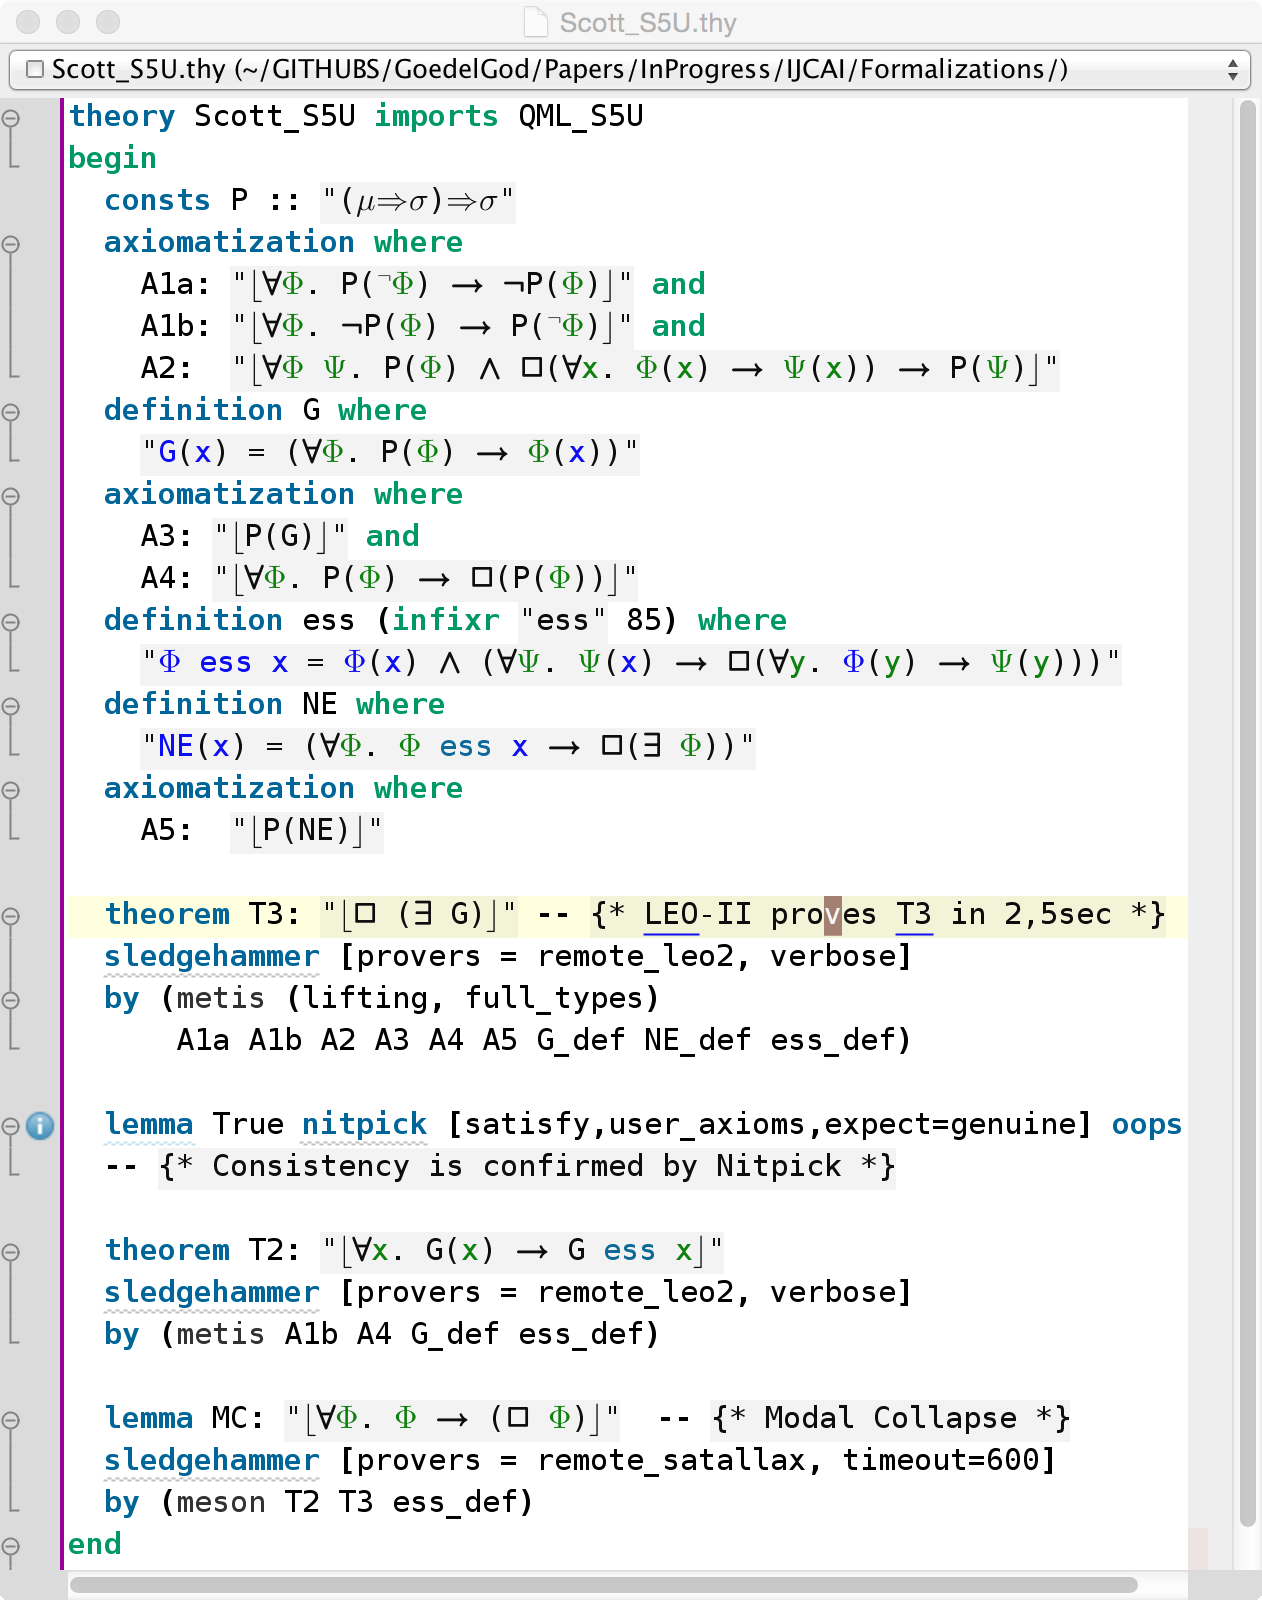
\includegraphics[width=\columnwidth]{./Images/Scott_S5U.png}}
\caption{Full Automation of T3 in \SFiveU; Consistency of Scott's
  Axioms;  Automatic Verification of Modal Collapse} \label{Scott_S5U}
\end{figure}
%\marginpar{ToDo: this picture has to be replaced by one without Isabelle errors}


\subsection{Improved Syntax in Isabelle}\label{sec:improvedsyntax}

Wider adoption of higher-order theorem proving technology for reasoning about and within embedded object logics, especially among non-expert users, is still hindered by the gap between the syntax used by people, when they write logical formulas with pen and paper, and the syntax used by higher-order logic theorem provers. Even when the syntax of the underlying higher-order system is elegant (as is the case in Isabelle/HOL), the embedding of HOML into HOL may easily expose details of HOL that may be uncommon to the user, disturbing his/her experience while using the system. To illustrate this point, Fig.~\ref{UglyEssence} shows how the definition of essence looked like in previous work \cite{J28}, where advanced syntax-sugaring features were not used. It looks notably higher-order, and its style differs significantly from the common style seen in works on modal logics and the ontological argument. The following specific issues can be enumerated:
\begin{enumerate}
\item Lambda abstractions (which are a typical higher-order feature) appear explicitly in places where it didn't need to appear in a pure HOML formulation (cf. G\"odel's manuscript, Fig.~\ref{GoedelScript}).
\item Quantifiers appear as higher-order dqefined constants, and not as binders. This forces the user to read (and write) formulas of the form $\forall (\lambda x. A(x))$ instead of the more common $\forall x. A(x)$.
\item The lifted modal connectives are represented by prefixing the
  letter ``m'' (e.g. $m\wedge$ and $m\imp$). The prefix disturbs the
  user, as it constantly reminds him/her that there is something
  unusual about the modal connectives.
\item Higher-order parenthesis conventions for the application of a predicate to a term are used. 
Instead of reading $\psi(y)$, as he would expect, he has to read $(\psi y)$. Outside niche areas in computer science, the former syntax is more widely known than the latter.
\end{enumerate}


\begin{figure}
\centerline{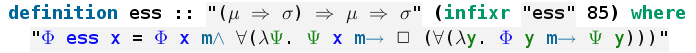
\includegraphics[width=\columnwidth]{./Images/UglyEssence.png}}
\caption{ Definition of Essence using Old Syntax } \label{UglyEssence}
\end{figure}

In the embedding presented here, in Fig.~\ref{QML_S5U}, advanced
syntax-sugaring effects provided by Isabelle were used to prevent
issues as enumerated above. The possibility to define boldface connectives allows us to drop the prefix; ``\texttt{binder}'' annotations enable modal quantifiers to be used in the standard binding way and reduce the need for explicit lambda abstractions; and a careful choice of priorities for infix connectives gives the parenthesis conventions that are more familiar to the user. As desired, the definition of essence in Fig.~\ref{Scott_S5U} is undeniably more immediately recognizable and comprehensible than the definition in Fig.~\ref{UglyEssence}. The embedding technique is now completely transparent to the user.

We hope that the syntax improvements described here will render the computer-assisted analysis of ontological arguments (as well as future works utilizing the embedding of modal logics into HOL) accessible to a wider audience and encourage philosophers to adopt logic-based artificial intelligence tools in order to conduct similar experiments in computational metaphysics.


\section{Intuitive Inconsistency Argument} \label{sec:inconsistency}

In the typical workflow of trying to prove a conjecture with a theorem prover, it is customary to check the consistency of the axioms first. For if the axioms are inconsistent, anything (including the conjecture) would be trivially derivable in classical logic (\emph{ex falso quodlibet}). Surprisingly, when this routine check was performed on G\"odel's axioms \cite{C40}, the \textsc{Leo-II} prover claimed that the axioms were inconsistent. Unfortunately, the refutation generated by \textsc{Leo-II} was barely human-readable. The text file was 153 lines\footnote{Long lines with an average of 184 characters per line.} long and machine-oriented proof calculus (higher-order resolution \cite{W47}) and syntax (TPTP THF \cite{J22}) were used. Part of the file is displayed in Fig.~\ref{LEO-Proof}.

\begin{figure*}
\centerline{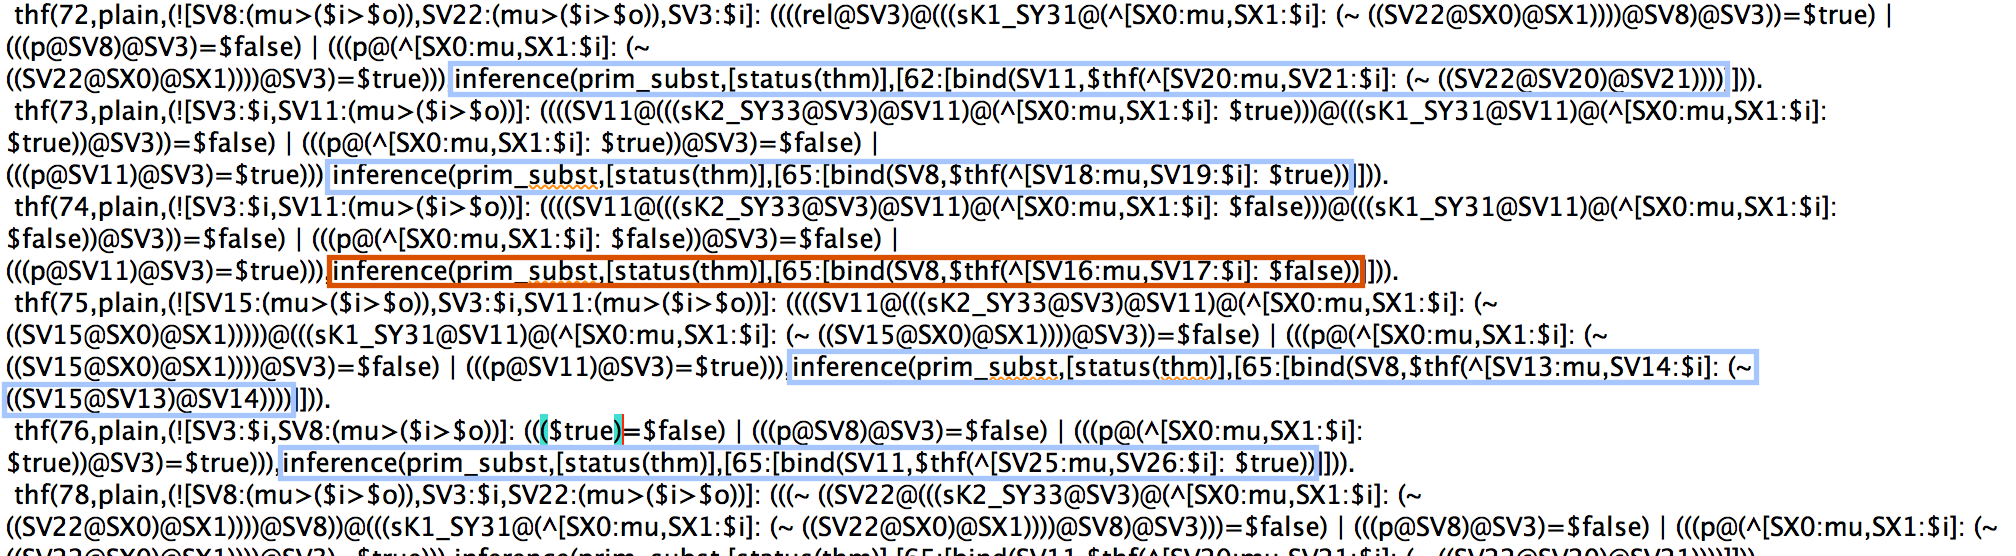
\includegraphics[width=\textwidth]{./Images/LEO-Proof.png}}
\caption{Lines 115--120 of \textsc{Leo-II}'s refutation. Primitive
  substitutions (e.g. with the empty property) are highlighted.} \label{LEO-Proof}
\end{figure*}

Although \textsc{Leo-II}'s resolution refutation is not easy to read
for humans, it did contain relevant hints to the importance of the
empty property $\lambda x. \bot$ (cf. Fig.~\ref{LEO-Proof}),
respectively, to self-difference $\lambda x.  x\not=x$. 

Note that both terms have identical denotations in a logic setting
with full functional and Boolean extensionality as given
here. Nevertheless, some philosophers may actually prefer the use of
self-difference over the empty property\footnote{This occurred e.g. in
  a private communication of the authors with Andr\'e Fuhrmann.} in
the analysis below. However, for the proof to go through it is
irrelevant which notion we use and the reader may simply replace the
empty property by self-difference.


% Philosophers
% might actually prefer using the latter variant over the
% former. However, on the given logic setting, with functional and
% Boolean extensionality, both terms have identical
% denotations. Consequently, they are mutually replacable below and the
% reader may simply use the version he prefers.

\subsection{Informal Argument}

Based on the hints found in \textsc{Leo-II}'s refutation, we conceived the following informal explanation for the inconsistency of G\"odel's axioms:

\begin{enumerate}
\item From G\"odel's definition of essence 
(${\ess{\phi}{x} \biimp {\allq \psi} (\psi(x)
\imp {\nec} \allq y (\phi(y) \imp \psi(y)))}$) it follows that the
empty property (or self-difference) is an essence of every individual (\textbf{Empty Essence Lemma}): 
$$\allq x\,(\ess{\emptyset}{x})$$

\item From theorem T1 (positive Properties are possibly
  exemplified: ${\allq \phi} [P(\phi) \imp {\pos}  \exq x
  \phi(x)]$) and axiom A5 (``necessary existence'' is a positive property: $P(\NE)$ ), it follows that $\NE$ is possibly exemplified:
  $$
  \pos \exq x [\NE(x)]
  $$
 
\item Expanding the definition of ``necessary existence''
  (${\NE(x) \equiv \allq \phi [\ess{\phi}{x} \imp \nec \exq y
    \phi(y)]}$), the following is obtained:
  $$
  \pos \exq x [\allq \varphi [ \ess{\varphi}{x} \imp \nec \exq y [\varphi(y)] ] ]
  $$

\item The sentence above holds for all $\varphi$ and thus, in
  particular, for the empty property (or self-difference):
$$
\pos \exq x [ \ess{\emptyset}{x} \imp \nec \exq y [\emptyset(y)] ]
$$

\item By the Empty Essence Lemma, the antecedent of the implication above is valid. Therefore, the sentence above entails:
$$
\pos \exq x [ \nec \exq y [\emptyset(y)] ]
$$ 

\item By definition of $\emptyset$: 
$$
\pos \exq x [ \nec \bot ]
$$

\item As the existential quantifier is binding no variable within its scope, the sentence is equi-valid with:
$$\pos \nec \bot $$

\item To see that the sentence above is contradictory, we may reason semantically, in terms of possible worlds. If $w_0$ is the arbitrary current world, the $\pos$ operator forces the existence of a world $w$ accessible from $w_0$ such that $\nec \bot$ is true in $w$. But $\nec \bot$ can only be true in $w$, if there is no world $w'$ accessible from $w$. In logics with a reflexive or symmetric accessibility relation (e.g. \KB), it is easy to see that there must be a world $w'$ accessible from $w$: either $w'$ itself, in case of a reflexive relation, or $w_0$, in case of a symmetric relation. In fact, even in \K, with no accessibility condition, there must be a world $w'$ accessible from $w$. The reason is that $\pos \nec \bot$ should be \emph{valid} (true in all worlds). Therefore, it is true in $w$ as well, where the existence of an accessible world $w'$ is forced by the $\pos$ operator. As a model for $\pos \nec \bot$ (which is a consequence of G\"odel's axioms) cannot be built, G\"odel's axioms are inconsistent.
\end{enumerate}

Interestingly, the refutation automatically generated by
\textsc{Leo-II} uses a symmetric accessibility relation, and thus
requires the modal logic KB. The informal, human-constructed
refutation described above, on the other hand, requires only the
weaker modal logic K. In our experiments \textsc{Leo-II} (like all
other HOL provers) was still to weak to automatically prove the
inconsistency already in logic K. Hence, this remains an open problem for automated
theorem provers.


\subsection{Argument Reconstruction in Isabelle}

To verify the correctness of the informal argument explained above, it was reconstructed in Isabelle/HOL, using Metis to automate the inessential parts. The essential use of the Empty Essence Lemma, on the other hand, is explicitly stated, to ensure that Isabelle is reconstructing the same argument. In fact, without the help of this lemma, Metis is not strong enough to refute G\"odel's axioms. \marginpar{ToDo: check this claim about Metis.}
\begin{figure}[t]
\centerline{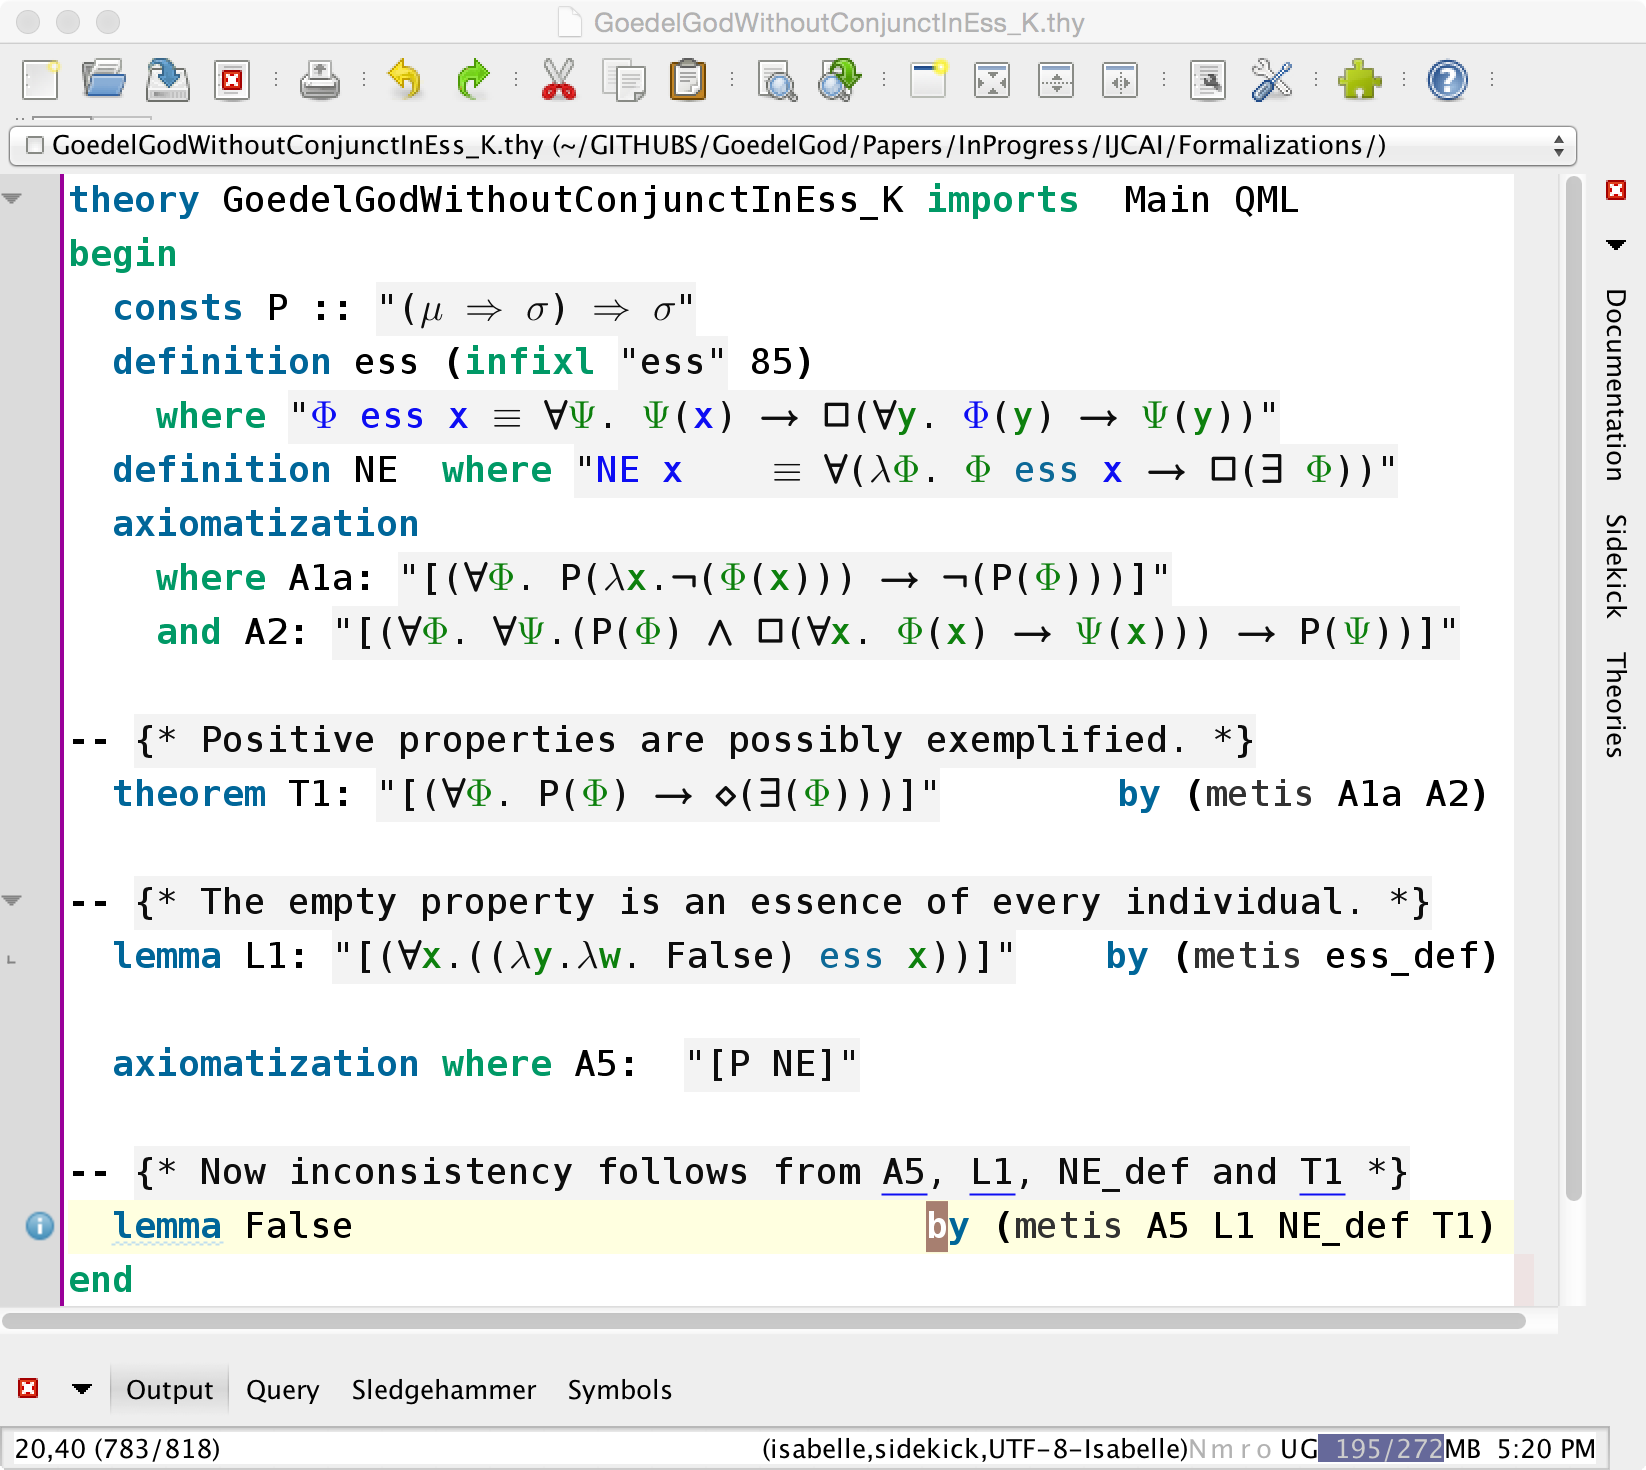
\includegraphics[width=\columnwidth]{./Images/InconsistencyIsabelleK.png}}
\caption{Refutation of G\"odel's Axioms in Isabelle/HOl..} \label{InconsistencyIsabelleK}
\end{figure}

\subsection{Mapping the Inconsistency to G\"odel}
The inconsistency verified in Fig.~\ref{InconsistencyIsabelleK} follows from the definition of
essence (ess), the definition of necessary existence (NE), the
axioms A1(a) and A2 (which entail theorem T1), and axiom A5. It remains to demonstrate that
these ingredients are actually present in G\"odel's manuscript in
Fig.~\ref{GoedelScript}. 

This can easily be seen: Axioms A1a in
Fig.~\ref{InconsistencyIsabelleK} is implied by Axiom Ax2 and the
highlighted footnote remark in Fig.~\ref{GoedelScript}. Axioms A2 and
A5 in Fig.~\ref{InconsistencyIsabelleK} correspond to Ax4 and Ax3 in
Fig.~\ref{GoedelScript}. The definitions of essence and necessary
existence are easy to identify. Thus, we conclude that the verified
inconsistency from Fig.~\ref{InconsistencyIsabelleK} does apply to 
G\"odel's original manuscript.


\section{Conclusion}\label{sec:conclusion}
The axioms and definitions in G\"odel's manuscript are inconsistent;
this has been detected automatically by the prover
\textsc{Leo-II}. Here we have presented a rational reconstruction and
verification of the inconsistency argument in Isabelle/HOL. This
argument is valid in all normal HOMLs including base logic K.
\begin{figure*}
\centerline{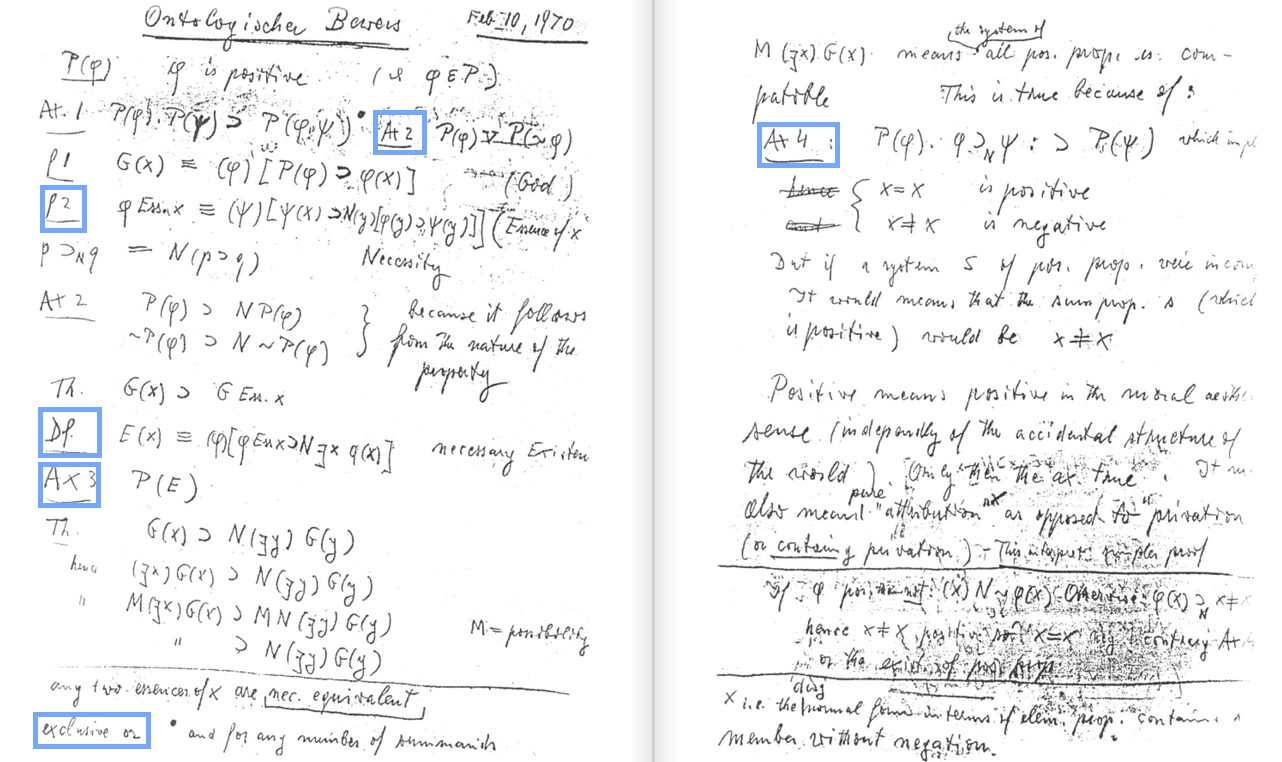
\includegraphics[width=\textwidth]{./Images/Manuscript2.png}}
\caption{G\"{o}del's manuscript, with mutually inconsistent axioms and definitions highlighted.} \label{GoedelScript}
\end{figure*}


We have also presented several technical improvements regarding the
semantic embedding approach. In particular, we have a achieved a
nearly perfect match between pen and paper presentations in HOML and
the syntax in Isabelle/HOL. As a result, the embedding of HOML in HOL
is now fully transparent and, as we think, ready for wider adoption by
philosophers.

On the other hand, there is still room for improvements. For example, Isabelle/HOL's Sledgehammer tool, which
orchestrates the calls to external automated theorem provers, such as
\textsc{Leo-II}, still fails to detect the inconsistency of G\"odel's
axioms, while a direct modeling of the problem in TPTP THF syntax in
combination with a direct call of \textsc{Leo-II} succeeds. In other
words, without independent experiments directly in TPTP THF the
inconsistency would thus not have been detected. There are further
technical issues regarding Sledgehammer that motivate
improvements. For example, in default setting, Sledgehammer does not
immediately inform the user when a proof has been found and instead silently
 first executes a series of time-consuming proof analysis processes (e.g. it's
dependency minimizer), before it eventually informs the user of success. For the
involved proof problems presented here (e.g. G\"odel's theorem T3:
\textit{Necessarily, there exists God}), this phase of silence may
take several minutes (during which the user might actually give up on
the proof attempt), while \textsc{Leo-II} already reported success to
Sledgehammer much earlier (e.g. after 2,5 seconds for T3).

Moreover, our work points to a challenge for proof transformation:
even if \textsc{Leo-II}'s proof can eventually be automatically
verified in Isabelle, without a human-intuitive explanation of the
proof, this will presumably be of limited value for philosophers.  The
challenge is to extract from such a verification process an abstract
level argument, similar to what we have presented in this paper: for
philosophers, the reconstruction of such human-intuitive arguments
from machine found proofs will likely be crucial for accepting any
novel results.

Another open problem that we solved in this paper is a fully automatic
proof of T3 directly from Scott's axioms. Again, this proof was
contributed by \textsc{Leo-II}. However, this has been possible only
after providing a more efficient embedding for HOML S5 in HOL. 

Both, the automated detection of the inconsistency in G\"odel's axioms
and the fully automatic proof of T3 from Scott's axioms demonstrates
the potential of our AI technology for philosophy: this technology is
in its current state of development already capable of contributing novel results to
metaphysics and to conduct reasoning steps at granularity-levels
beyond common human capabilities.


% Good improvement (technical sense), Sledgehammer can still be improved
% (\textsc{Leo-II} finds inconsistency when call directly in THF Syntax, but not
% from within Isabelle). 


% We also point to several technical challenges which, at least for the
% moment, still restrain non-expert users of these systems from
% independently conducting similar experiments in computational
% metaphysics as reported here and in previous work.


% Technical issues detected within Isabelle-Sledgehammer; room for improvements



\section*{Acknowledgments}

Will be added at a later point.

%German Research Foundation DFG, Chad Brown






\small 
%% The file named.bst is a bibliography style file for BibTeX 0.99c
\bibliographystyle{named}
\bibliography{Bibliography}

\end{document}

